\documentclass[]{article}
\usepackage[a4paper, total={15cm,23cm}]{geometry}
\usepackage{fancyhdr}
\usepackage{graphicx}
\usepackage{amsmath}
\usepackage{amssymb}
\usepackage{xcolor}
\usepackage{verbatim}
%opening
\title{PH 223 Week 3}
\author{Benjamin Bauml and Danielle Skinner}
\date{Winter 2024}
\pagestyle{fancy}
\rhead{PH 223}
\chead{Winter 2024}
\lhead{Week 3}

%Custom Quotation Command
\newcommand{\excerpt}[1]{\colorbox{lightgray}{\parbox{14.8cm}{#1}} \\}

\begin{document}

\maketitle

\begin{center}
Problems 1 and 2 are borrowed/adapted from Chapter 24 of the \textit{Student Workbook} for \textit{Physics for Scientists and Engineers}. An integral from Activity 3 comes from the inside cover of \textit{Classical Mechanics} by John R. Taylor.
\end{center}
\section*{Activity 1}%3,4
\excerpt{
The figures shown below are cross sections of three-dimensional closed surfaces. They have a flat top and bottom surface above and below the plane of the page. However, the electric field is everywhere parallel to the page, so there is no flux through the top or bottom surface. The electric field is uniform over each face of the surface. The field strength, in N/C, is shown.
}
\excerpt{
(1.1) For each, does the surface enclose a net positive charge, a net negative charge, or no net charge?
}
\begin{center}
	%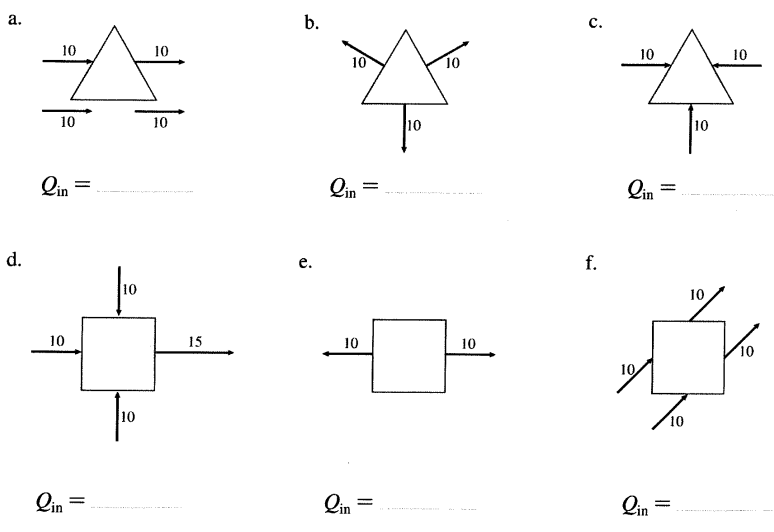
\includegraphics[scale=0.5]{A11}
	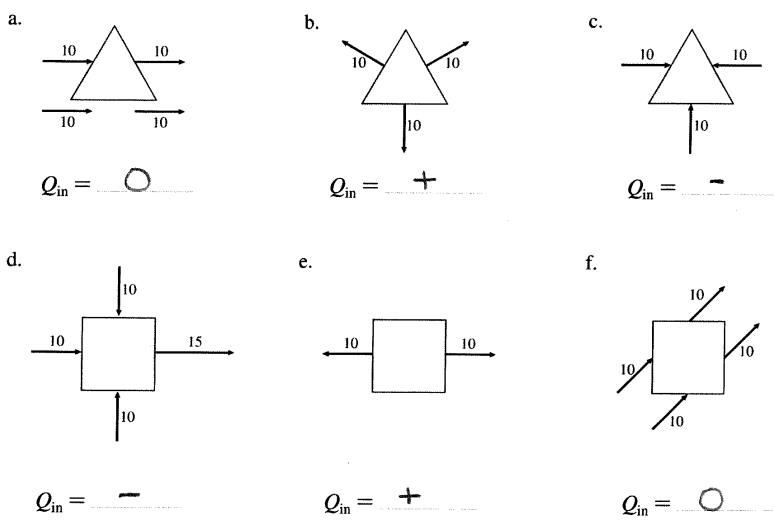
\includegraphics[scale=0.5]{A11Sol}%Solution
\end{center}
\pagebreak
\excerpt{
(1.2) Each surface contains no net charge. Draw the missing electric field vector (or write $ \vec{E} = \vec{0} $) in the proper direction. Write the field strength beside it.
}
\begin{center}
	%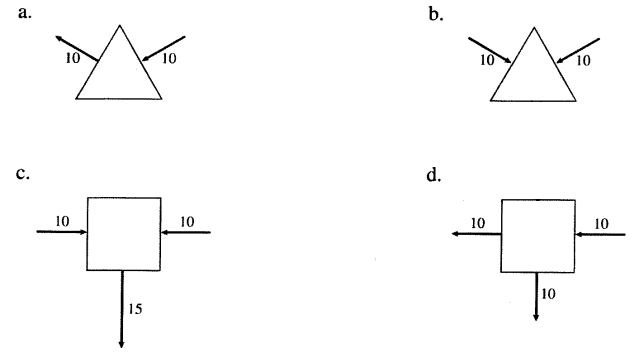
\includegraphics[scale=0.5]{A12}
	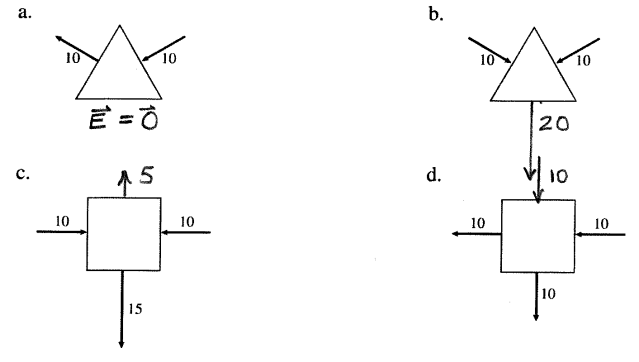
\includegraphics[scale=0.5]{A12Sol}%Solution
\end{center}
\vspace{-40pt}

\section*{Activity 2}%9
\excerpt{
A uniform electric field is shown below.
}
\begin{center}
	%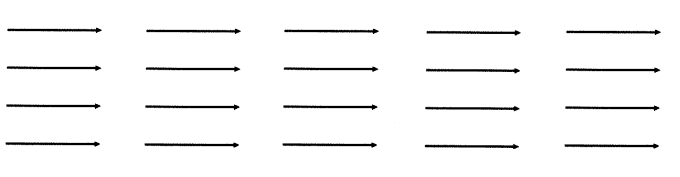
\includegraphics[scale=0.5]{A2}
	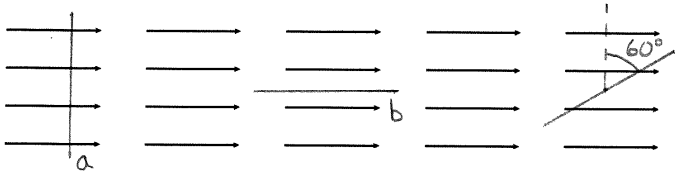
\includegraphics[scale=0.5]{A2Sol}%Solution
\end{center}
\excerpt{
Draw and label an \textit{edge view} of three square surfaces, all the \textit{same size}, for which \\
(a) The flux is maximum. \\
(b) The flux is minimum. \\
(c) The flux has half the value of the flux through the square part of (a). \\
Give the tilt angle of any squares not perpendicular or parallel to the field lines.
}
For part (c), we want the flux through the surface to be half of the flux through the surface in part (a):
\[
\Phi_{c} = \frac{1}{2}\Phi_{a}.
\]
The flux through surface $a$ is
\[
\Phi_{a} = \vec{E}\cdot\vec{A} = \left|\vec{E}\right|\left|\vec{A}\right|\cos(0) = \left|\vec{E}\right|\left|\vec{A}\right|,
\]
because the area vector and electric field vectors are parallel. The flux through surface $c$ is
\[
\Phi_{c} = \vec{E}\cdot\vec{A} = \left|\vec{E}\right|\left|\vec{A}\right|\cos(\theta).
\]
Using our first equation, we can solve for $\theta$:
\[
\begin{split}
	\left|\vec{E}\right|\left|\vec{A}\right|\cos(\theta) & = \frac{1}{2}\left|\vec{E}\right|\left|\vec{A}\right| \\
	\cos\theta & = \frac{1}{2}.
\end{split}
\]
This happens when $\theta=\frac{\pi}{3}$, or for an angle of 60$^{\circ}$. Note that $\theta$ is defined as the angle between the area vector and the electric field vectors, while the above picture indicates the angle between the surface and the vertical. This is still accurate---turning the area vector 60$^{\circ}$ down from the horizontal means the surface is being turned 60$^{\circ}$ right of the vertical.

\pagebreak
\section*{Activity 3}
\excerpt{
You have a point charge $ Q > 0 $ a distance $ L $ below the center of a horizontal square surface with sides of length $ 2L $. What is the flux through the surface?
}
\excerpt{
(a) First, what is the electric field due to the point charge? Express this in Cartesian coordinates, then specify what the field is through the plate.
}
% To reveal the solution, delete "\phantom{\parbox{\textwidth}{" from the beginning, and "}}" from the end.


In general, the electric field of a point charge at the origin is
\[
\vec{E} = \frac{KQ}{r^{2}}\hat{r} = \frac{KQ}{r^{3}}\vec{r}.
\]
In terms of Cartesian coordinates, this is
\[
\vec{E} = \frac{KQ}{(x^{2}+y^{2}+z^{2})^{3/2}}(x\hat{\imath}+y\hat{\jmath}+z\hat{k}).
\]
If the electric field is at the origin, let us put the plate in the $ z = L $ plane, with its sides at $ x = \pm L $ and $ y = \pm L $. As such, the electric field through the plate is
\[
\vec{E}(z=L) = \frac{KQ}{(x^{2}+y^{2}+L^{2})^{3/2}}(x\hat{\imath}+y\hat{\jmath}+L\hat{k}).
\] \\
\excerpt{
(b) Choose a unit normal for the surface, then evaluate the quantity $ \vec{E}\cdot d\vec{A} $ using this surface normal and the coordinate system you plan to integrate in.
}
% To reveal the solution, delete "\phantom{\parbox{\textwidth}{" from the beginning, and "}}" from the end.
For an open surface, there is no prescribed unit normal vector, but let us choose $ \hat{k} $ (pointing up and away from the charge). The area element is therefore $ d\vec{A} = \hat{k}dxdy $. It follows that
\[
\begin{split}
	\vec{E}(z=L)\cdot d\vec{A} & = \left(\frac{KQ}{(x^{2}+y^{2}+L^{2})^{3/2}}(x\hat{\imath}+y\hat{\jmath}+L\hat{k})\right)\cdot\hat{k}dxdy \\
	& = \frac{KQL}{(x^{2}+y^{2}+L^{2})^{3/2}}dxdy \\
\end{split}
\]
\excerpt{
(c) Set the bounds on your integral to find the flux. Using $ \int\frac{dx}{(1+x^{2})^{3/2}} = \frac{x}{(1+x^{2})^{1/2}} $, evaluate one integral of the expression. Do not attempt the second integral. \\
}
%\begin{comment}
Given how we placed the sides in part (a) (with the $ z $-axis through the center of the plate), both integrals run from $ -L $ to $ L $:
\[
\Phi_{e} = \int_{-L}^{L}\int_{-L}^{L}\frac{KQL}{(x^{2}+y^{2}+L^{2})^{3/2}}dxdy.
\]
We can rearrange this to be of the form of the given integral:
\[
\Phi_{e} = KQL\int_{-L}^{L}\frac{1}{(y^{2}+L^{2})^{3/2}}\int_{-L}^{L}\frac{dx}{(x^{2}/(y^{2}+L^{2}) + 1)^{3/2}}dy.
\]
Making the substitution $ x' = x/\sqrt{y^{2}+L^{2}} $, we end up with the integral
\[
\begin{split}
	\Phi_{e} & = KQL\int_{-L}^{L}\frac{1}{y^{2}+L^{2}}\int_{-L/\sqrt{y^{2}+L^{2}}}^{L/\sqrt{y^{2}+L^{2}}}\frac{dx'}{(x'^{2} + 1)^{3/2}}dy = KQL\int_{-L}^{L}\frac{1}{y^{2}+L^{2}} \left[\frac{x'}{(1+x'^{2})^{1/2}}\right]_{x'=-L/\sqrt{y^{2}+L^{2}}}^{L/\sqrt{y^{2}+L^{2}}} dy \\
	& = KQL\int_{-L}^{L}\frac{1}{y^{2}+L^{2}} \left[\frac{L}{(y^{2}+2L^{2})^{1/2}} - \frac{-L}{(y^{2}+2L^{2})^{1/2}}\right] dy = KQL\int_{-L}^{L}\frac{2L}{(y^{2}+L^{2})(y^{2}+2L^{2})^{1/2}} dy \\
\end{split}
\]
We appear to be rather stuck here. However, if we recognize that our surface is one side of a cube enclosing charge $ Q $ (hence my choosing $ \hat{k} $, which would have been the outward normal), Gauss' law implies it should have one sixth of the total flux $ \frac{Q}{\epsilon_{0}} = 4\pi KQ $. That would mean $ \Phi_{e} = \frac{4\pi}{6}KQ $.
%\end{comment}

\end{document}
